\documentclass[journal]{IEEEtran}
\usepackage{fontspec}
\setmainfont{Times New Roman}
\setsansfont{Arial}
\usepackage{amsmath,amssymb,graphicx,booktabs,tabularx,array,url}
\usepackage[hidelinks]{hyperref}\usepackage{microtype}
\setlength{\emergencystretch}{2em}
\newcommand{\Range}{\operatorname{Range}}
\title{When Does a Current Mode Affect a Material Update?\\Feedback and Bidirectional Transfer in Inverse Scattering}
\author{Manuscript for technical discussion}
\begin{document}\maketitle
\begin{abstract}
A current direction influences a material inverse update through material excitation, multiple-scattering feedback, and reception. For a specified Galerkin current-space change, we expose the retained feedback and factor the Jacobian change into observation and injection signatures. Their paired material pullbacks contain the complete regularized Gauss--Newton step change. The change acts on both data curvature and the residual-dependent normal-equation term, so increased information volume need not improve the step. This mechanism leads to receiver-centered conditional exchange: retain a receiver-derived backbone, rank actual model-induced displacements using a richer reduced reference, and check finalists on the complete frozen quadratic using cached output and directional tangent actions. In three-dimensional vector-Maxwell tests on four geometries with Gaussian and voxel material spaces, at most three exchanges improve 35 of 36 state--budget cases and leave one unchanged. The median object-summed quadratic-gap ratio is 0.348, a 65.2\% reduction at unchanged current dimension. Aggregating one-decision gains at each object's common checkpoints, full-dictionary proxy ranking captures 98.1--99.6\% of the best local one-decision gain; restricted candidate coverage explains the largest missed opportunities. Maxwell witnesses also show increasing information volume with negative step gain and positive joint gain from two unfavorable singleton additions. Complete costs and earlier Krylov controls locate the practical limits: these results establish a conditional current-design method for accurate frozen material updates, with candidate acquisition, output-error certification, and nonlinear transfer determining its deployment value.
\end{abstract}

\begin{IEEEkeywords}Electromagnetic inverse scattering, induced currents, multiple scattering, material sensitivity, current subspaces, conditional model selection.\end{IEEEkeywords}
\section{Introduction}
Electromagnetic inverse scattering infers a material distribution from the fields it scatters. The measurements are generated by induced currents inside the object, so representing these currents is a natural way to organize the inverse problem. A reduced current space can greatly simplify a forward model. The question for material inversion is more specific: which of its current directions must be represented accurately to obtain the material update?

A receiver measures the radiation of the entire interacting object. The direct radiation of an individual current direction is only part of that response. That direction can excite other currents, which scatter again and radiate toward the receiver. Moreover, a material change can excite only those currents permitted by the local total field and the chosen material variables. These two facts identify the route by which a current direction can matter: material excitation must reach it, and its interacting response must return to the measured channels. Its effect on the actual step also depends on the data residual and regularization.

This paper makes that test precise for a specified change in a current approximation. At the same material state, illumination, residual, admissible material tangent, and regularization, we enlarge an existing Galerkin current space. Eliminating its retained coordinates reveals the multiple-scattering feedback accompanying every added direction. The resulting Jacobian change separates into a receiver-observation factor and a material-injection factor. Their two material pullbacks contain the complete change in the regularized Gauss--Newton step.

The paired support identifies where the change can occur; its coefficients and alignment with the complete objective determine whether it is useful. An enlarged current model approximates the same measurements, rather than adding independent observations. Its curvature increment can therefore be indefinite. At a fixed current budget, we make this distinction actionable by replacing a small number of receiver-based directions. Each replacement changes both material data curvature and the residual-dependent normal-equation term. A larger information-volume score need not generate a better material step.

The paper connects three levels of evidence. The operator factorization explains the electromagnetic entry and return paths and the exact material-step support. Vector-Maxwell witnesses resolve retained feedback missed by direct radiation. A bounded receiver-centered exchange experiment then separates local opportunity, reduced-reference ranking, directed validation, and their costs. It evaluates the displacement actually generated by a new current model on the unchanged complete quadratic. Cached output and one directional tangent action per finalist provide the scalar check without a new full adjoint. Earlier equal-budget and structural-repair failures remain controls for this interpretation. Standard elimination, least-squares identities, low-rank inverse formulas, and information summaries support the argument; the physical content lies in the current pathways and their material-update consequences.

\section{Background: From Observable Currents to Material Updates}
\subsection{What current-subspace methods already provide}
For a prescribed induced current, the exterior Green operator maps that current to measured scattered fields. Its singular vectors separate well-observed from weakly observed current components. The subspace-based optimization method (SOM) uses this structure together with the material/current consistency equation. Twofold SOM also analyzes the internal Green operator, and FFT-TSOM constructs efficient Fourier current spaces. Subspace-based distorted-Born methods update the background field while exploiting deterministic current information \cite{r17,r1,r2,r3,r16}. Thus internal propagation and material consistency are already central to this literature.

Our question concerns the consequence of modifying a particular current space at a particular material state. The material derivative contains both the state-dependent total field and the multiple-scattering resolvent. The present result complements observation and propagation structure by tracing a specified current-space modification through this state-dependent material tangent into the local material normal equation. Our SOM- and TSOM-inspired candidate banks isolate the role of current-space selection within a common material solver; native nonlinear optimizer comparisons are outside this experiment.

\subsection{The relation to reduced models and Krylov methods}
Primal/dual reduced models can preserve outputs and parameter derivatives when the required solution directions are included \cite{r4}. Goal-oriented reduction and adaptive parameter-identification methods likewise use task information to guide approximation \cite{r5,r6,r9}. We use these established ideas in the electromagnetic setting, where material injection, dyadic propagation, and transverse reception have distinct physical meanings.

A Krylov method builds material directions by repeated action of the complete regularized curvature. Augmentation and deflation reuse selected directions to improve subsequent solves \cite{r8}. Material-space reuse provides a direct numerical benchmark for the value of current-derived preconditioning. We compare a two-level material inverse applied throughout PCG with the current-derived inverse, under matched histories, storage budgets, and stopping quality.

\subsection{A feedback interpretation}
The current equation contains a frequency-domain feedback loop: currents create an internal field, and the material converts that field into further currents. For an added current direction, one branch radiates directly; the other enters the retained current space and returns after its internal interactions. The feedback diagram represents this frequency-domain algebraic elimination: the loop is closed by the material response and internal Green propagation.

\begin{figure*}[t]\centering
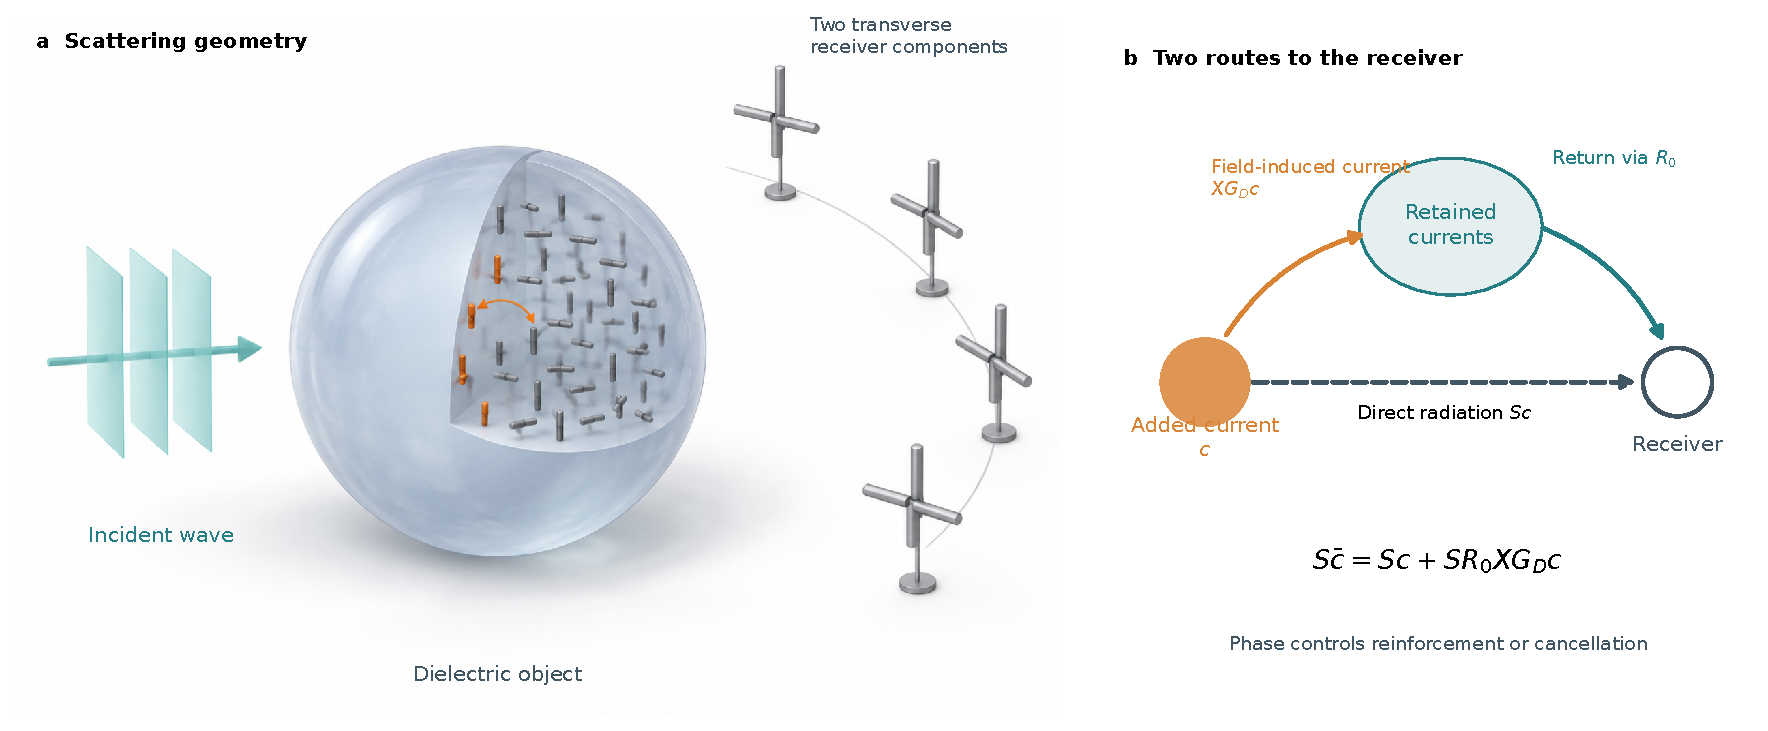
\includegraphics[width=.95\textwidth]{figures/physical_feedback.pdf}
\caption{Material excitation, internal feedback, and reception in a finite dielectric object. The direct radiation of an added current is only one route to the receiver; the retained currents can carry an additional response. The drawing is a conceptual geometry, not a computed field distribution.}
\end{figure*}
\section{Electromagnetic Entry, Feedback, and Observation}

\subsection{Physical tangent and frozen inverse problem}

Consider isotropic, nonmagnetic dielectric contrast \(\chi\) with a fixed acquisition geometry. For illumination \(p\), the contrast-source formulation is

\[
\begin{aligned}
j_p&=X(e_p^{\rm inc}+G_Dj_p),&
L&=I-XG_D,\\
L\,\delta j_p&=B_ps,&
B_ps&=DX[Q_Ts]e_p^{\rm tot}.
\end{aligned}\tag{1}
\]

Here \(G_D\) is the internal vector Green operator; \(X\) is the material response; \(e_p^{\rm tot}\) is the current total field; and \(Q_T\) expands a real material coordinate vector \(s\in\mathbb R^d\), including both parts of complex contrast. Thus \(d\) is the admissible real material dimension. Its realified expansion obeys \(Q_T^\top M_\chi Q_T=I\), with the volume-weighted material \(L^2\) metric \(M_\chi\). Current coordinates are also normalized to their declared discrete metric. With the receiver/scaling map \(S\),

\[
K_p=L^{-1}B_p,\qquad J_p=SK_p. \tag{2}
\]

The actual DDA uses contrast-dependent polarizability, rather than substituting \(X=\chi\) in its discrete equation. Its injection retains the polarizability derivative and the vector local field; Supplement S1 gives the exact implemented model. The operator identities use \(A=I-L\); \(A=XG_D\) expresses their contrast-source interpretation, and \(A=D_aG_{\rm off}\) is the implemented DDA counterpart.

Illuminations have separate currents and one shared material vector $s\in\mathbb R^d$. Each excitation $B_ps$ produces a current change $L^{-1}B_ps$ and measurement change $J_ps$. Stacking $[\operatorname{Re}(J_ps);\operatorname{Im}(J_ps)]$ over illuminations gives one real measurement vector. The normal equations are therefore real material-space equations, with $^*$ denoting the corresponding adjoint. The complex current-block identities lift through block-diagonal current operators and vertically stacked material injection (Supplement S1).

At a frozen state, let \(r\) be predicted minus observed data, \(\Lambda\succ0\) the common regularization/damping curvature, and \(\ell\) its common linear prior term. Define the full relative quadratic

\[
\begin{aligned}
\Phi(s)&=\frac12\|r+Js\|^2-\frac12\|r\|^2\\
&\quad+\frac12s^*\Lambda s+\ell^*s\\
&=\frac12s^*Hs+h^*s,\\
H&=J^*J+\Lambda,& h&=J^*r+\ell.
\end{aligned}\tag{3}
\]

Thus \(\Phi(0)=0\), \(s_*=-H^{-1}h\), and the squared \(H\)-energy step error is twice the full quadratic gap, providing an exact measure of local step quality.

\subsection{Specified Galerkin enlargement}

Let \(V\) be an orthonormal current basis, \(C\) an orthonormal candidate bank with \(V^*C=0\), and assume \(V^*LV\) is invertible. The old Galerkin operators are

\[
\begin{aligned}
R_0&=V(V^*LV)^{-1}V^*,& K_0&=R_0B,\\
J_0&=SK_0,& H_0&=J_0^*J_0+\Lambda,\\
&&M_0&=H_0^{-1}.
\end{aligned}\tag{4}
\]

\(R_0\) solves a retained current equation; \(M_0\) solves a material normal equation. Put

\[
\begin{aligned}
\bar C&=(I-R_0L)C=C+R_0AC,& Y_C&=S\bar C,\\
N_C&=C^*(B-LK_0),& \Gamma_C&=C^*L\bar C.
\end{aligned}\tag{5}
\]

The symbol \(\Gamma_C\) denotes a current Schur matrix and is distinct from the receiver map \(S\). For \(A_{UV}=U^*AV\), \(D_V=I-A_{VV}\), \(B_V=V^*B\), and \(B_C=C^*B\), these factors become

\[
\begin{aligned}
\bar C&=C+VD_V^{-1}A_{VC},\\
Y_C&=SC+(SV)D_V^{-1}A_{VC},\\
N_C&=B_C+A_{CV}D_V^{-1}B_V,\\
\Gamma_C&=I-A_{CC}-A_{CV}D_V^{-1}A_{VC}.
\end{aligned} \tag{6}
\]

\textbf{Proposition 1 (feedback-dressed tangent factorization).} If \(\Gamma_C\) is invertible, the strictly Galerkin tangent in \([V,C]\) satisfies

\[
K_C-K_0=\bar C\Gamma_C^{-1}N_C,\qquad
\Delta J:=J_C-J_0=Y_C\Gamma_C^{-1}N_C. \tag{7}
\]

\textbf{Proof.} The enlarged coefficient matrix has blocks \(D_V,-A_{VC},-A_{CV},I-A_{CC}\). Eliminating its retained coordinates gives \(\Gamma_C\) and right-hand side \(N_C\). Back-substitution adds \(VD_V^{-1}A_{VC}\) to the raw candidate response \(C\), proving (6)--(7). It also gives \(V^*L\bar C=0\). \hfill\(\square\)

Equation (6) identifies three physical paths. First, an added current radiates directly through \(SC\), but also generates an internal field through \(G_D\), excites retained currents through \(X\), and radiates through \(SV\) after retained-space rescattering. Hence

\[
\boxed{\bar C=C+R_0XG_DC}
\]

in the contrast-source formulation. Second, material injection can enter the retained space through \(B_V\) before reaching the new coordinates through \(A_{CV}\). Third, \(A_{CV}D_V^{-1}A_{VC}\) is the added-to-retained-to-added loop, which enters the Schur inverse rather than a single-pass correction. The dressed current preserves the retained Galerkin equations through \(V^*L\bar C=0\), while generally losing Euclidean orthogonality to \(V\). For a receiver-dark candidate, the isolated direct branch \(SC\) is zero or near roundoff; internal scattering produces the nonzero dressed response \(S\bar C\).



\subsection{Weak relative feedback requires more than weak scattering}

If \(\|A_{VV}\|\le\eta<1\), a sufficient absolute bound is

\[
\|Y_C-SC\|\le
\frac{\|SV\|\,\|A_{VC}\|}{1-\eta}. \tag{8}
\]

To obtain a direction-uniform \emph{relative} bound on a candidate subspace, its direct radiation must also be bounded away from zero. If \(SC\) is injective there, then

\[
\frac{\|(Y_C-SC)a\|}{\|SCa\|}
\le\frac{\|SV\|\,\|A_{VC}\|}
{(1-\eta)\sigma_{\min}(SC)}
\quad(a\ne0). \tag{9}
\]

A singular \(SC\) requires restriction to a specified non-dark coefficient space. A sufficient Schur-invertibility condition is \(\|A_{CC}+A_{CV}D_V^{-1}A_{VC}\|<1\). These sufficient conditions separate weak absolute coupling from weak relative feedback. Small absolute feedback may dominate a nearly dark direct response; cross-space coupling and a large, possibly nonnormal retained resolvent provide additional amplification mechanisms. Their contributions must be resolved before attributing a large ratio to resonance.

\section{Paired Material Closure and Nonmonotone Curvature}

\subsection{The two-channel regularized step change}

Set \(T_C=\Gamma_C^{-1}N_C\). For the same \(B,r,\Lambda,\ell\), define

\[
\begin{aligned}
s_0&=-M_0(J_0^*r+\ell),\\
s_C&=-(J_C^*J_C+\Lambda)^{-1}(J_C^*r+\ell),\\
\mathcal E_0(C)&=\operatorname{Range}M_0[J_0^*Y_C,N_C^*].
\end{aligned}\tag{10}
\]

\textbf{Theorem 1 (paired step-change closure).} Under Proposition 1, with exact actions, positive regularization, and no nonzero signature removed,

\[
\begin{aligned}
s_C-s_0={}&-M_0J_0^*Y_C(T_Cs_C)\\
&-M_0N_C^*\Gamma_C^{-*}Y_C^*(r+J_Cs_C)
\in\mathcal E_0(C).
\end{aligned} \tag{11}
\]

\textbf{Proof.} Write \(\Delta H=J_C^*J_C-J_0^*J_0\) and \(\Delta h=\Delta J^*r\). Expanding \(J_C=J_0+Y_CT_C\) gives

\[
\Delta H=J_0^*Y_CT_C+T_C^*Y_C^*J_0+T_C^*Y_C^*Y_CT_C.
\]

Subtract the normal equations: \(H_0(s_C-s_0)=-\Delta Hs_C-\Delta h\). Collect the first observation term and the remaining \(T_C^*Y_C^*(r+J_Cs_C)\) term, and use \(T_C^*=N_C^*\Gamma_C^{-*}\). \hfill\(\square\)

The observation lift \(M_0J_0^*Y_C\) redistributes the update along old sensitivities when they couple to the added response. The injection lift \(M_0N_C^*\) pulls the updated data residual back through the new current excitation. Looking only at \(\Delta h\) retains the second channel and can miss the first channel's Hessian coupling.

The factors identify the available routes for material influence, while the coefficients in (11) determine how the present residual activates them. For example, when $r=0$ and $\ell=0$, both regularized steps vanish regardless of the derivative change. This separates structural coupling from its activation in a particular inverse step.

\subsection{Why one side is generally insufficient}

The exact illustration

\[
J_0=[1,0],\quad J_C=[1,1],\quad \Lambda=I,\quad r=1,\quad\ell=0
\]

gives \(s_0=(-1/2,0)^\top\), \(s_C=(-1/3,-1/3)^\top\), and \(s_C-s_0=(1/6,-1/3)^\top\). The observation lift is along the first material coordinate and the injection lift along the second. Neither alone contains the change. Although \(\Delta J=[0,1]\) has rank one,

\[
\Delta H=\begin{bmatrix}0&1\\1&1\end{bmatrix},\qquad\det\Delta H=-1. \tag{12}
\]

Both \(H_0=J_0^*J_0+\Lambda\) and \(H_C=J_C^*J_C+\Lambda\) remain positive definite under \(\Lambda\succ0\). The indefinite difference \(\Delta H\) describes redistribution of material curvature between these two well-posed regularized problems.

This algebraic illustration embeds in \(L=I\) Galerkin reduction (Supplement S3). It isolates the least-squares effect: two-sided material coupling can occur even without scattering feedback. Feedback determines the electromagnetic factors; material least squares supplies the two-channel normal coupling.

\section{What the Transfer Geometry Can Guarantee}
The paired space describes the material change caused by a specified current enlargement. Optimizing in that space and reducing the error of a complete material step are different tasks. For a material correction $d$ from a step $x$, the complete objective gain is $-g_F(x)^Td-d^TH_Fd/2$. Thus even a large, accurately represented current contribution can point away from the present full-model defect.

There is a corresponding complete-tail identity. For $R_U=U(U^*LU)^{-1}U^*$, set $\mathcal I_U=(I-LR_U)B$ and $\mathcal O_U=S(I-R_UL)$. Direct multiplication gives
\[
 J-J_U=\mathcal O_U L^{-1}\mathcal I_U.
\]
An omitted response must connect the material injection side to the observation side through the interacting current equation. The factors are residual operators, not independent scalar weights. Without a bound on $L^{-1}$, their norms alone do not certify a small material error.

This geometry has also been used to construct a material inverse for complete normal-equation solves. The low-rank inverse realization and the standard PCG spectral consequences are given in the supplement. In this paper they provide a design comparison, rather than an additional solver contribution: a structural repair space can lose to material Krylov directions, and preconditioning can save iterations while losing total time. The current-selection test below instead fixes the actual current dimension and asks whether changing the model improves the material step itself.

\section{Conditional Current Exchange and the Value of a Material Step}
\subsection{Changing a current model changes two material quantities}
A receiver-based space provides a reproducible starting approximation. At a fixed current budget, we can replace one of its directions while retaining the others. This asks a local design question: does the replacement improve the material step generated by the model? The test keeps the material state, illumination, physical tangent, residual, prior term and damping fixed.

Let the old and new current spaces be $[V,A]$ and $[V,C]$. When the common-core and Schur systems are invertible, their Jacobian difference is
\begin{equation}\label{eq:exchange-difference}
 D=Y_C\Gamma_C^{-1}N_C-Y_A\Gamma_A^{-1}N_A.
\end{equation}
These are two changes relative to the same retained core. If that core is singular, stable endpoints may still exist; then we compute the endpoints directly rather than using this elimination.

In the common real material coordinates, write $\mathsf I_U=J_U^TJ_U$ for the data curvature. This differs from the injection residual used in the tail identity. A current change alters both data curvature and the constant gradient term:
\begin{equation}\label{eq:information-offset}
\begin{aligned}
 \Delta\mathsf I&=J_o^TD+D^TJ_o+D^TD,\\
 h_U&=J_U^Tr+\ell,\qquad \Delta h=D^Tr.
\end{aligned}
\end{equation}
Here the normal equation is $H_Us_U=-h_U$. The data curvature describes which material changes produce a measured response. The constant term describes how those responses align with the present residual. Both determine the actual endpoint step difference:
\begin{equation}\label{eq:exchange-step}
 d=s_n-s_o=-H_n^{-1}(\Delta h+\Delta\mathsf I s_o).
\end{equation}
The formula follows by subtracting the two normal equations. It applies to the fixed unconstrained quadratic; changing an active constraint set requires its own optimality equations.

Information magnitude alone cannot select this step. Even the scalar models $J_o=1$ and $J_n=-1$ have identical data curvature but opposite steps for $r=1$, $\ell=0$ and $\Lambda=1$. More generally, $\Delta\mathsf I$ can be indefinite: changing the approximation to existing data includes interference terms, unlike adding independent measurements.

\subsection{Evaluate the displacement actually produced}
For the unchanged full quadratic, a proposed displacement $d$ from $x$ has signed gain
\begin{equation}\label{eq:exchange-gain}
 Q=\Phi_F(x)-\Phi_F(x+d)=-g_F(x)^Td-\tfrac12d^TH_Fd.
\end{equation}
Positive gain means a better approximation to this frozen full-model material update. It does not by itself determine material truth error. The latter also contains a cross term with the unknown material error, and nonlinear reconstruction additionally requires feasible updates and step acceptance.

The scalar gain can be checked without a new full adjoint. Cache $u=r+J_Fx$ and compute $z=J_Fd$. Then
\begin{equation}\label{eq:directional-exchange-gain}
 Q=-u^Tz-(\ell+\Lambda x)^Td-\tfrac12(\|z\|^2+d^T\Lambda d).
\end{equation}
For complex data the first product is $\operatorname{Re}\langle u,z\rangle$. Each full directional action still pays for every illumination. After an accepted move, the endpoint and conditional candidate scores change; the cached output updates as $J_Fx\leftarrow J_Fx+z$.

If validated output-error bounds $e_u,e_z$ are available, the computed gain has error at most
\begin{equation}\label{eq:exchange-gain-bound}
 \epsilon_Q=e_u\|\widehat z\|+(\|\widehat u\|+\|\widehat z\|)e_z+e_ue_z+\tfrac12 e_z^2.
\end{equation}
A positive lower bound can justify acceptance. A local stopping certificate instead requires an upper bound below tolerance for every feasible move in the declared neighborhood. A shortlist with no accepted move does not establish that condition. The computations below use double-precision full directional checks; a rigorous output bound is unavailable, so their numerical acceptance and stopping status are reported separately.

\subsection{Information diagnostics and their scope}
We normalize data curvature with a fixed positive material scale $P$, kept separate from numerical Levenberg--Marquardt damping. For eigenvalues $\nu_i$ of $P^{-1/2}\mathsf I_UP^{-1/2}$, we record
\begin{equation}
 d_{\rm eff}=
 \sum_i\frac{\nu_i}{1+\nu_i},\qquad
 \mathcal D=\tfrac12\sum_i\log(1+\nu_i).
\end{equation}
These quantities summarize the response claimed by a model. We also measure its curvature discrepancy from the full reference. Greater $\mathcal D$ need not mean greater fidelity, and neither scalar retains the residual-dependent term in~\eqref{eq:information-offset}. The present data normalization is a prescribed numerical scale, not an independently calibrated noise covariance; no mutual-information interpretation is needed.

Small Gaussian material spaces permit complete reference diagnostics. For the larger voxel spaces, all endpoints use the same sixteen material probe directions; those information measures describe that projection only. Information diagnostics, full-reference steps and material truth remain evaluation data, separate from the reduced-reference scores used to propose exchanges.

\section{Maxwell Evidence and the Limits of Structural Repair}
\subsection{Physical model and independent reference}
The finite-object computations use three-component Maxwell DDA with six transverse illuminations and two transverse receiver components. Material coordinates are real, including both parts of complex contrast, and orthonormalized in the volume-weighted material metric. The DDA injection retains $a'(\chi)E^{\rm tot}$ for the contrast-dependent polarizability $a$, rather than treating polarizability as contrast. The supplement gives the exact dyadic, self-term convention, material gauge, and real adjoint.

All principal calculations use FP64. Algebraic checks compare block elimination with direct Galerkin endpoints, their material steps, and the complete directional gain. Rank deficiency, complex phase and permutation changes, singular common cores, and CPU/CUDA consistency are included. Implementation consistency and continuum fidelity are checked separately.

A homogeneous sphere of radius 0.35, wavenumber 2, and contrast $1+0.05i$ provides an independent vector-Mie reference. At the finest $32^3$ grid the aggregate complex far-field error is 0.252\% and the uniform real-contrast derivative error is 0.731\%. Grid errors are nonmonotone; this validates the stated sphere response and uniform perturbation, not every voxel Jacobian direction. The coarse high-contrast sphere retains its 21.40\% independent discrepancy.

\subsection{Direct radiation can miss retained feedback}
Three constructed two-column current banks on $5^3$, $6^3$, and $7^3$ free-space grids have direct receiver norms below $1.7\times10^{-16}$. Their feedback-dressed norms are 0.0672, 0.0720, and 0.0888; their material derivative discrepancies are respectively 3.56\%, 3.98\%, and 5.22\% of the full Jacobian norm. A seeded material tangent generates the candidate currents, which are projected outside the receiver-row and retained-current spaces. These discrete witnesses isolate the additional route carried by retained currents. They establish existence, rather than its frequency among arbitrary current directions.

\begin{figure*}[tbp]\centering
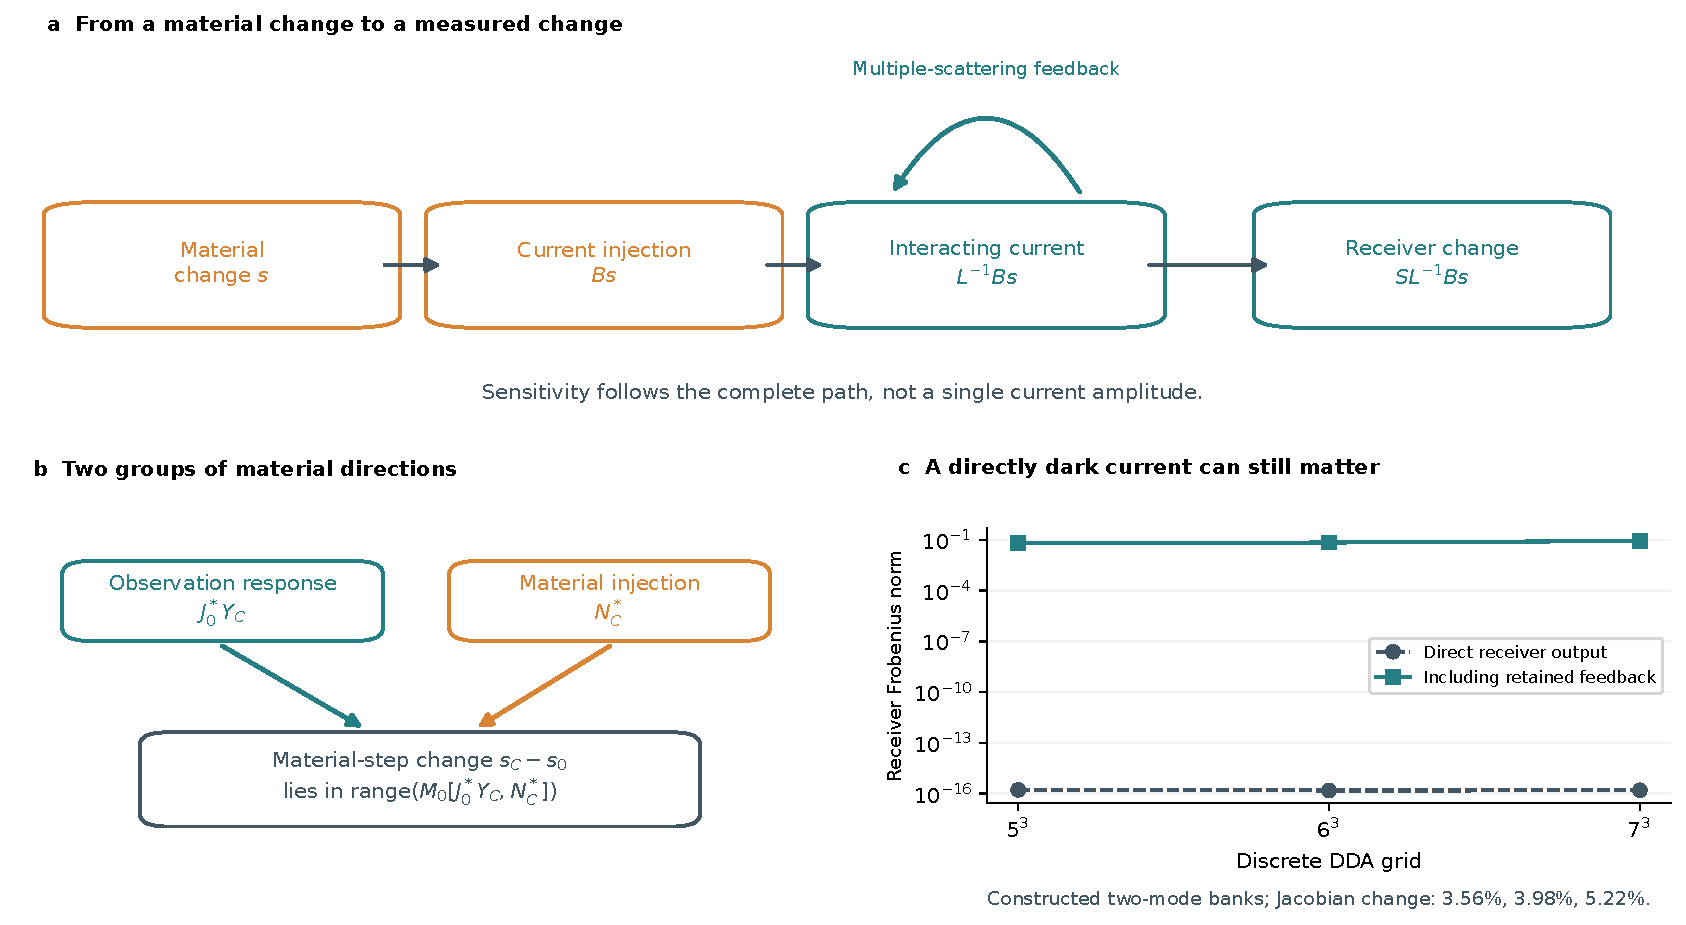
\includegraphics[width=.91\textwidth]{figures/material_paths.pdf}
\caption{A material perturbation enters the current equation and returns to the receivers through the interacting response. The numerical panel compares direct and retained-feedback outputs of constructed free-space Maxwell currents. The small direct output is at FP64 roundoff; the feedback response is resolved within the discrete model.}
\end{figure*}

\subsection{Closure, optimization, and cost give different answers}
Paired material repair reduces full-quadratic error more than its specified direct current enlargement in all 72 smooth and all 36 sharp frozen-state comparisons. Equal-real-rank material Krylov correction is better than paired repair in every one of those comparisons. Thus exact step-change support does not identify the best equal-rank correction for the complete objective.

Five normalized closure checks miss their original tolerance, with absolute $H$-distance $1.06\times10^{-15}$--$3.43\times10^{-14}$. Their Schur condition numbers are 1.00020--1.00093. The precision traces support cancellation and small-denominator amplification, rather than ill-conditioned Schur inversion or established underflow. All five failed checks remain in the record.

The paid paired warm-start route costs 1.416 times matched ordinary PCG, and increases full-wave RHS from 66 to 342. A separate current-derived preconditioning use obtains eight-use cost ratios 0.773--0.877 across six objects when the history is already paid. Charging dedicated history acquisition makes all six ratios exceed one; cached Ritz recycling wins on two objects. These results distinguish physical structure from an economical way to acquire it.

The four sharp-target reconstructions also retain substantial relative material errors, 0.755, 0.750, 0.560, and 0.906. They constrain claims about interface recovery for that acquisition. The conditional exchanges below reuse frozen states and do not create new nonlinear reconstruction evidence.

\subsection{Equal current dimension: opportunity and access}
The previous preconditioning tests solve the same complete normal equation. We next test the current approximation itself. All selectors use a common full forward residual, total-field material injection, physical material coordinates, and regularization; only the tangent-current Galerkin space changes. The budget $k=4,8,12,16,24,32$ is the actual number of independent complex current columns shared across six illuminations. The quality measure is the gap in the unchanged full quadratic, as defined in the preceding design section.

Sixteen prescribed objects cover smooth Gaussian lobes, touching or separated ellipsoids, shell/layered structures, and asymmetric multiple objects. Each family has two Gaussian and two voxel material tangents. The inverse and data grids are $12^3$ and $14^3$; receivers provide two transverse channels at 64 positions. The latter grid is a finer DDA reference. Initial, pre-fourth-update, and final valid linearizations come from one common full-reference trajectory per object. One reference failed and two state evaluations ended in native process failures. The observed noiseless subset therefore contains 43 of 48 states, 258 of 288 state--budget units, and 15 objects; 13 objects have all three states. Deferred noise checks and these gaps retain their original status.

Receiver singular vectors, a projected receiver/internal proxy, Fourier directions, current-energy POD, and ten random seeds supply current-based controls. Transfer-magnitude, lifted joint-spectrum, first-order gain, and finite-gain rules share the declared candidates. The finite rules estimate full-quadratic gain using an independent 64-column current reference, with zero or limited complete-model probes. Each addition is rescored with full Schur coupling. A generic primal--dual current POD/Galerkin adaptation uses the same information and total dimension. Separately charged offline search evaluates actual current Galerkin spaces in a declared dictionary union, including tested baseline spaces; it is best-found rather than globally certified.

For each object we sum paired absolute gaps and divide by the corresponding receiver sums, then report the median of object ratios. The receiver rule was locked using development data. Intervals use 10,000 object-cluster bootstrap replicates; states and budgets are repeated observations within each object. The offline search achieves ratio 0.4242, with 95\% interval $[0.2832,0.5710]$. Both finite-gain variants have ratio 1.0947 and win on six of 15 objects. The no-probe interval is $[0.3814,1.8308]$; the limited-probe interval is $[0.3814,1.8601]$. Their median captured fraction of resolvable same-domain oracle improvement is $-0.1396$, retained without clipping. Searching with complete information demonstrates opportunity; the tested reduced-reference rule does not reliably recover it.

\begin{table}[tbp]\centering\caption{Observed noiseless object-median full-quadratic gap ratios relative to development-locked receiver selection at the same actual current dimension. Smaller is better. The search is offline; both finite rules are separately evaluated.}\label{tab:current-budget}
\footnotesize\setlength{\tabcolsep}{3pt}\begin{tabular}{rrrrr}\toprule
$k$ & \shortstack{Finite\\no probes} & \shortstack{Limited\\probes} & \shortstack{Offline\\search} & \shortstack{Primal--dual\\POD}\\\midrule
4 & 0.480 & 0.480 & 0.396 & 3.597\\
8 & 1.185 & 1.200 & 0.574 & 4.824\\
12 & 1.937 & 1.937 & 0.519 & 3.393\\
16 & 4.216 & 4.216 & 0.620 & 4.527\\
24 & 5.296 & 5.296 & 0.521 & 1.882\\
32 & 5.611 & 5.604 & 0.327 & 0.861\\\bottomrule
\end{tabular}\end{table}

\begin{figure*}[tbp]\centering
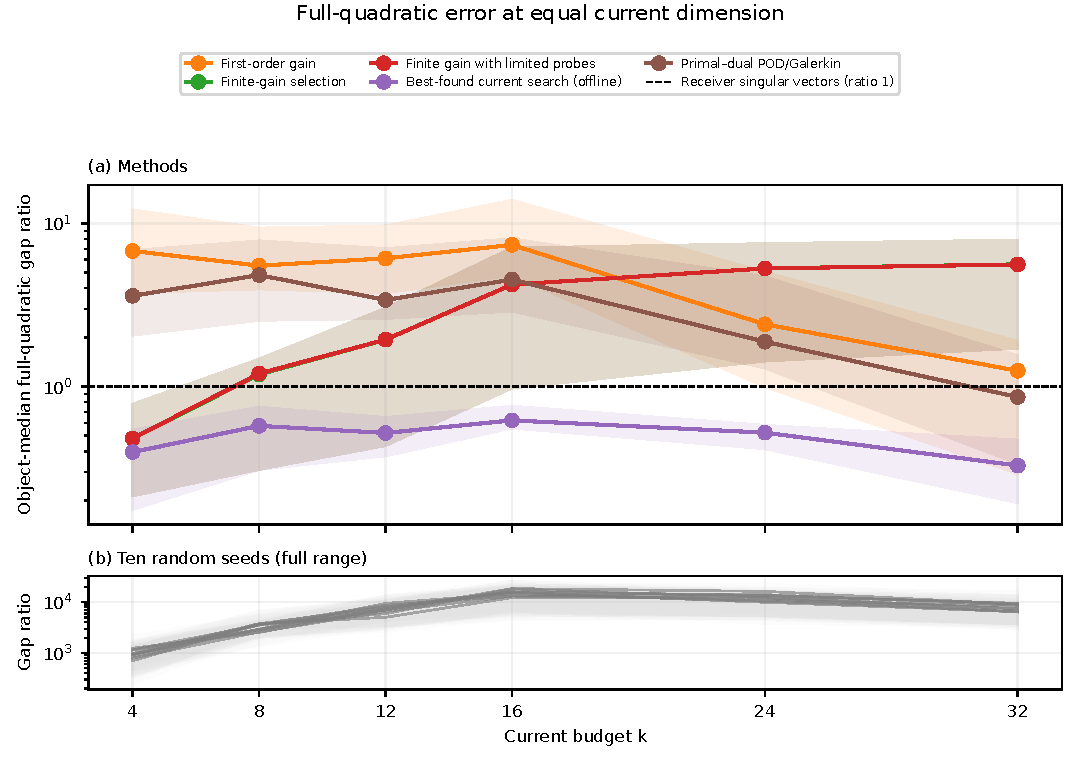
\includegraphics[width=.94\textwidth]{figures/current_design/01_fullgap_ratios.pdf}
\caption{Full-quadratic step error at equal actual current dimension. The upper panel shows object-median ratios and frozen 95\% intervals; the lower panel retains all ten random seeds over their complete range. The two finite-gain curves mostly overlap and are evaluated separately. They help at $k=4$ but lose their relative advantage as the tested budget increases. Offline current search remains below the receiver reference. These are 43 noiseless observed states from 15 objects, with missing states retained in coverage. FP64-equivalent implementation versions are combined for accuracy, while their costs remain separated.}
\label{fig:current-design}
\end{figure*}

The predeclared phase summaries also expose useful local regimes. The no-probe ratio is 1.2761 at initialization, 0.2793 before the fourth update, and 0.3597 at the last saved state. The asymmetric family ratio is 0.2793, whereas Gaussian-lobe and shell-family ratios are 1.3481 and 1.5843. These slices describe where the tested rule helps; they do not replace the failed aggregate criteria. Restricting the sensitivity analysis to the 13 complete objects leaves the finite/receiver median unchanged.

Against the particular primal--dual POD adaptation, the finite rules have aggregate ratio 0.2904 (95\% interval $[0.0785,0.5649]$). The finite/first-order policy ratio is 0.1171, but the policies also differ in their displacement and terminal swap procedure. This ratio therefore does not isolate the quadratic penalty. The controlled displacement-by-evaluation comparison below addresses those factors at the same checkpoint. The receiver control is stronger overall, and the primal--dual comparison reverses at larger budgets. No new selector reconstruction was launched because the aggregate frozen-state criteria and planned coverage were not satisfied. The supplement reports every tested control, absolute gaps, reference floors, missing cells, and version-specific marginal fees.

\section{Conditional Exchange: Opportunity, Ranking, and Cost}
\subsection{Receiver-centered conditional exchange protocol}
We use two development geometries, a near-contact object with Gaussian material coordinates and a layered object with voxel coordinates. A fixed extension uses a smooth Gaussian object and an asymmetric multi-object voxel target. Each supplies the initial, third-update, and seventeenth-update linearizations, with shared complex current dimensions $k=4,8,16$. The four objects therefore give 36 correlated state--budget cells. All reuse existing noiseless trajectories; states and budgets are not independent objects.

At each state a declared dictionary combines 32 receiver directions, 32 internal-propagation directions, 32 Fourier directions, 32 reduced primal--dual directions, 16 residual-current directions, and ten seeded random currents. Its 154 atoms have a lossless common embedding of rank 128. That embedding caches $L,S,B$ projections; the retained model still has exactly $k$ columns. This is a newly declared dictionary, not the original selector experiment's dictionary. The 1-swap teacher enumerates all feasible replacements in this domain: 600, 1168, and 2208 at the receiver starting spaces for $k=4,8,16$. It is a complete local enumeration, not a global optimum over all current subspaces.

The online proposal uses twelve incoming atoms, balanced across source families without complete-objective labels, and considers each deletable logical atom. It computes endpoint steps and reduced-anchor gains from a separate 64-column model. It then checks at most two finalists by the complete directional formula, accepts a resolved positive gain, and recomputes the conditional neighborhood. At most three actions are accepted. The exact-score teacher, unchecked surrogate, verified proposal, unchanged receiver, and a deletion/addition/swap policy with rank at most $k$ are recorded separately. A fixed restricted 2-swap domain supplies interaction diagnostics. Singular common cores trigger direct endpoint evaluation; endpoint stability determines feasibility.

The material state, full forward residual, injection, prior term $\ell$, damping, and physical coordinates are common to all methods. Full Jacobians and full-reference optimal steps are used only for offline diagnostics. Gaussian spaces have 54 real material coordinates; voxel spaces have 3456. The former allow complete information spectra, while voxel information diagnostics use sixteen fixed common directions. The material scale is $P=10^{-5}I$, separately recorded from LM damping. No measured noise covariance is fitted.

The reported risk is the complete frozen-quadratic gap relative to the paid reference solve. Its reference residual and floating-point floor accompany every cell. Ratios first sum paired risks within each object and only then aggregate objects. The numerical acceptance tolerance is predeclared; it is not a rigorous output-error bound. Selector construction, rejected candidates, failed factorizations, directed RHS, teacher labels and information diagnostics have separate cost records.

\subsection{A receiver-centered neighborhood has resolved opportunity}
All twelve planned states and 36 state--budget cells completed. At unchanged current dimension, the median object-summed risk ratio of the verified method is 0.348, corresponding to a 65.2\% reduction. The local teacher reduces object-summed risk to 0.0984--0.2016 of unchanged receiver selection. The directed-verified proposal improves 35 cells and leaves one unchanged, with no numerically resolved deterioration. Its four object ratios are in Table~\ref{tab:exchange-objects}. These are noiseless frozen-step results on four existing objects, with correlated states and budgets.

\begin{table}[tbp]\centering\caption{Object-summed complete-quadratic risk ratios. Each denominator sums the nine unchanged-receiver cells of the same object.}\label{tab:exchange-objects}
\begin{tabular}{@{}lrrr@{}}\toprule
Geometry / material space&Teacher&Verified&Gain capture\\\midrule
Smooth / Gaussian&.0984&.1904&89.8\%\\
Near-contact / Gaussian&.2016&.6538&43.4\%\\
Layered / voxel&.1520&.2776&85.2\%\\
Asymmetric / voxel&.1628&.4181&69.5\%\\\bottomrule
\end{tabular}
\par\smallskip\footnotesize Gain capture is the ratio of verified and teacher risk reductions along their respective three-action paths; it is descriptive and differs from same-checkpoint ranking regret.
\end{table}

\begin{figure*}[tbp]\centering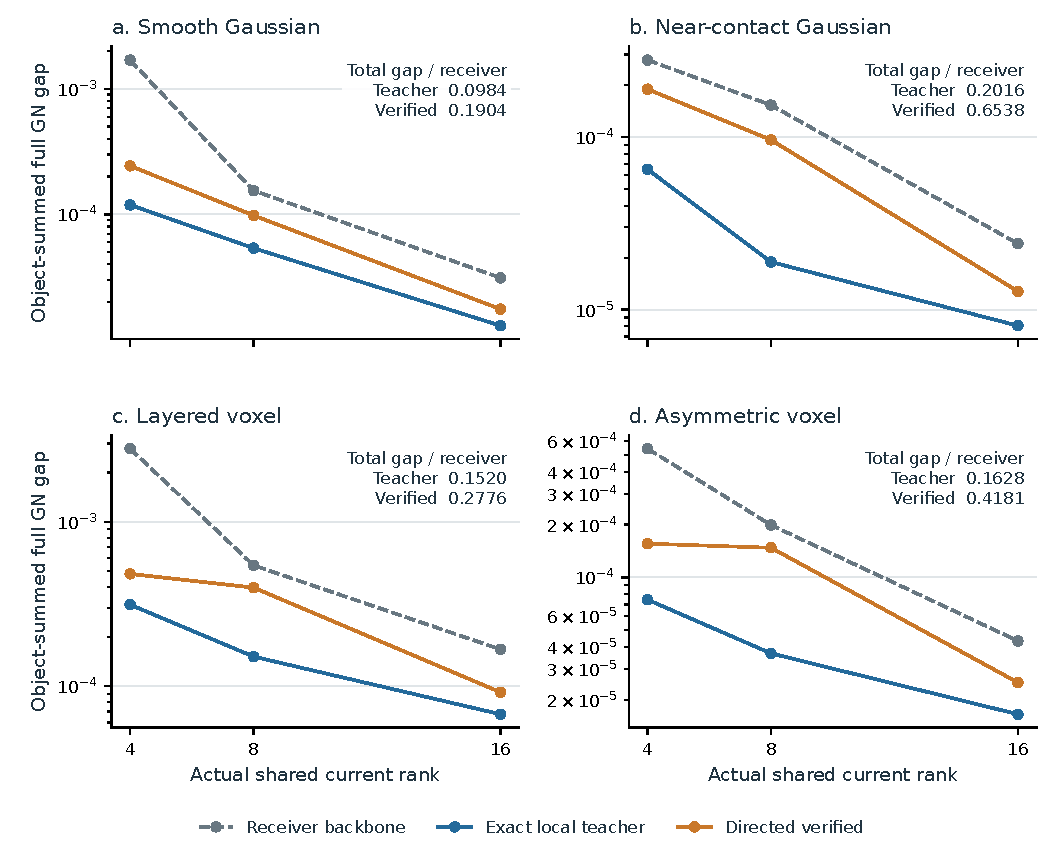
\includegraphics[width=.92\textwidth]{figures/exchange_risk.pdf}
\caption{Absolute complete-quadratic gaps summed over three states of each object at each current budget. The teacher exhausts a declared local exchange neighborhood; the verified method sees twelve incoming candidates and checks at most two finalists per round. The curves are descriptive object summaries, not 36 independent objects or nonlinear reconstruction errors.}
\end{figure*}

We separate proposal error from omitted opportunity at the common receiver checkpoint. With the full dictionary available, anchor top-one ranking captures 98.1--99.6\% of the object-summed best one-decision gain. The twelve-incoming pool contains 35.3\%, 91.98\%, 96.89\%, and 65.89\% of that opportunity for the near-contact, layered, smooth, and asymmetric objects. The near-contact result is therefore mainly a shortpool limitation at this checkpoint, rather than a large full-dictionary ranking error. This diagnosis does not equate differing multi-action paths with pure score regret.

The rank-at-most-$k$ policy ends at $k$ in every cell. It produces a different path in one case but demonstrates no terminal rank saving. Verified exchanges accept 75 actions, paying 1164 finalist tangent RHS in addition to the separately recorded initialization and screening costs. Twenty-two cells stop unresolved and fourteen reach their move budget. No complete-neighborhood stopping certificate is established.

\subsection{Information growth can accompany a worse step}
Information diagnostics cover a fixed twelve-incoming subset per removal, with the teacher-best move separately added when absent. Complete information spectra are available on the Gaussian material spaces; voxel metrics use the common sixteen-direction projection. The augmented diagnostic subset is utility-biased and is not a prevalence sample of all current directions.

For one resolved near-contact initial-state replacement at $k=4$, information volume increases by 6.3127 and effective dimension by 1.8613, while the actual complete-quadratic gain is $-5.5754\times10^{-5}$. The normalized curvature fidelity also improves slightly. Thus neither information magnitude nor this fidelity scalar determines the signed update utility. Equation~\eqref{eq:information-offset} identifies the missing residual-dependent term.

\begin{figure*}[tbp]\centering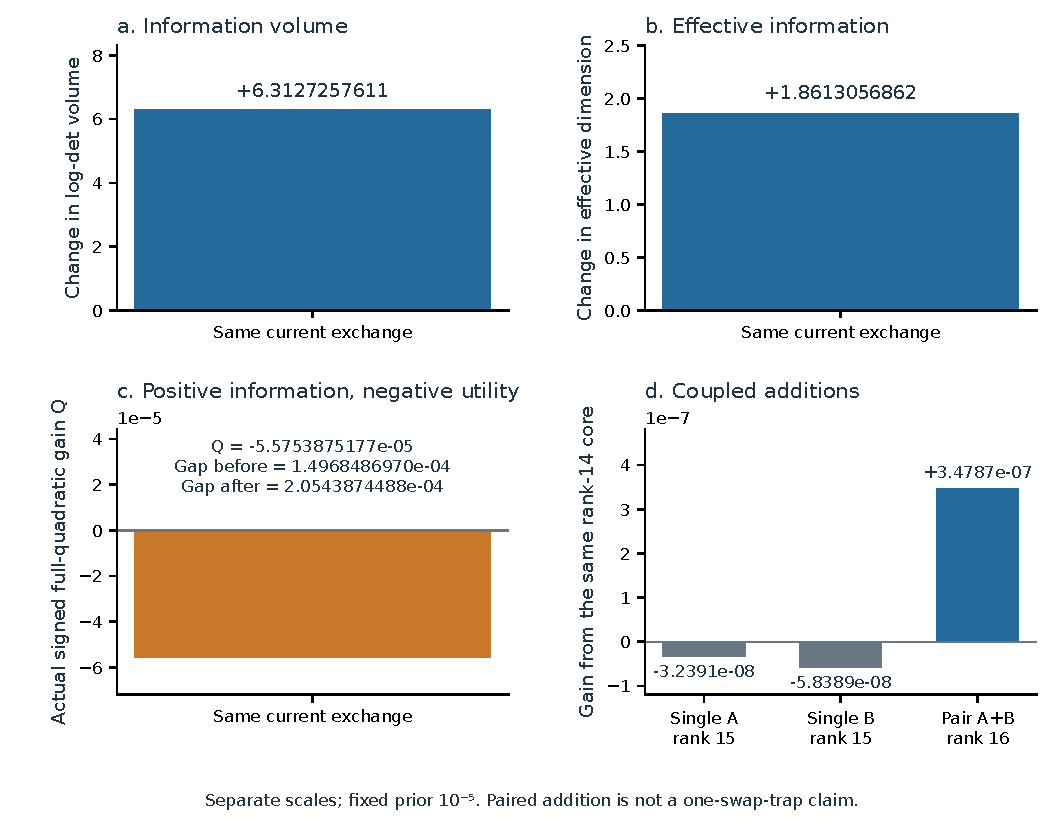
\includegraphics[width=.90\textwidth]{figures/information_and_pair_witness.pdf}
\caption{Left: a physical Maxwell replacement increases both information-volume and effective-dimension diagnostics but worsens the actual material step. Separate axes retain their different units. Right: from a common rank-14 core, two rank-15 singleton additions have negative gain, while their rank-16 joint addition has positive gain. This is an addition-interaction witness, not a same-rank 1-swap trap.}
\label{fig:information-pair}
\end{figure*}

Five strict joint-addition witnesses occur in the 540 fixed-core pair tests. One has singleton gains $-3.2391\times10^{-8}$ and $-5.8389\times10^{-8}$, but joint gain $3.4787\times10^{-7}$. Candidate coupling can therefore defeat independent singleton decisions. On a separate common-candidate diagnostic, mandatory top-one selection using linear evaluation of actual displacement chooses negative-gain endpoints in 29 of 36 cells; complete quadratic evaluation reduces this count to one. Scoring a linearized displacement and executing the actual endpoint also retains substantial mismatches. The deployed acceptance includes no-op and rejects negative gains. This controlled diagnostic replaces a causal interpretation of the older, confounded finite/first-order policy ratio.

\subsection{What the checks cost and what remains untested}
Two representative early states use the same CUDA FP64 endpoint and physical direction-action backend for five rotated timing repetitions. Median warm selection time for the conditional method is 0.594, 1.418, and 2.690~s on the near-contact Gaussian state at $k=4,8,16$, and 0.891, 1.153, and 3.400~s on the layered voxel state. One directed decision using the same initial shortpool costs 0.328--0.937~s and 0.333--1.215~s, respectively. The cached fixed-onepass control costs 0.113--0.219~s and has different proposal semantics. Conditional verification buys fidelity with additional screening and physical actions; these timings establish no acceleration over unchanged receiver selection. Historical cache acquisition is separately recorded, while independent cold speedup remains unmeasured.

A fixed two-architecture, three-seed CPU priority pilot uses object-grouped train/validation/test partitions. On the single heldout asymmetric object, MLP top-two opportunity capture is 98.85--99.16\%; group-mean capture is 75.99--98.03\%. Every run is below anchor top-two capture, 99.885\%. These labels evaluate offline priority, with no new physical acceptance test or measured all-in feature-cost saving. Learned proposal is therefore not retained as an algorithmic contribution.

The full-reference Gaussian direction decomposition reproduces archived risk changes to relative error below $6.5\times10^{-11}$. All six Gaussian states have zero full-reference weak directions under the declared threshold $\nu\le1$ and scale $P=10^{-5}I$. Weak directions suggested by a reduced model cannot be treated as verified full-material prior freedom. The voxel projection cannot resolve weakness in the entire material space.

Finally, the unconstrained unit-step truth diagnostic improves material error relative to the current state in 19 cells and worsens it in 17; 28 steps violate the material constraints. No nonlinear exchange reconstruction is run. The evidence supports conditional frozen-update design, with output-error certification, economical proposal construction, noise, and accepted nonlinear transfer remaining open.

\section{Design Implications}
\subsection{Preserve a reliable backbone, then test a specific change}
The four-object exchange study gives a constructive answer to the paper's question. Receiver ordering provides a useful starting space; a few conditionally evaluated replacements substantially improve the complete material step without increasing its current dimension. The 35 resolved improvements and the median 65.2\% object-level gap reduction demonstrate local design value across both tested material representations. The operative quantity is the gain of the displacement produced by the modified model. Neither its direct radiation nor its transfer norm supplies that sign.

This design preserves what the receiver model already does well. A candidate is evaluated relative to the remaining currents, including their feedback and mutual coupling. After accepting a move, the current endpoint step, cached output, and conditional factors are updated before choosing another. The method consequently uses physical structure to decide a bounded model modification, rather than treating a current ranking as independent of the selected space or the present residual.

\subsection{Candidate coverage is an actionable bottleneck}
After summing one-decision gains over each object's nine common receiver checkpoints, the richer-reference score captures 98.1--99.6\% of the best gain in the declared neighborhood. Yet the twelve-incoming pool contains only 35.3\% of that opportunity for the near-contact object and 65.9\% for the asymmetric object. Improving proposal coverage is therefore a more direct next design task than replacing an already accurate full-dictionary score with a more elaborate regressor. The six learned-priority runs reinforce this reading: all trail the analytical anchor top-two rule on the heldout object.

Coverage and conditional interaction must be considered together. The positive-pair Maxwell witnesses show that two unfavorable singleton additions can jointly help. These witnesses motivate limited block proposals when a singleton screen is inconclusive; they do not supply a universal greedy or submodularity guarantee. The complete teacher comparison remains local to its declared dictionary and action horizon.

\subsection{Information structure and update utility are distinct}
Increasing a model's information volume can enlarge its curvature while changing its residual pullback in the wrong direction. The resolved replacement in Fig.~\ref{fig:information-pair} increases information volume and effective dimension and slightly improves the measured curvature fidelity, yet worsens the complete material step. This is an electromagnetic example of why both terms in Eq.~\eqref{eq:information-offset} are needed. Information diagnostics explain which directions change; signed full-quadratic gain decides whether the current task benefits.

All information comparisons use fixed physical material coordinates and the declared scale. Statistical Fisher or posterior interpretations additionally require an appropriate noise and prior model. The present normalized data scale is a numerical convention. The Gaussian full-reference spectrum has no weak direction at the specified threshold, while the voxel projection samples only sixteen material directions. These findings guide the weak-material gate without establishing a global voxel posterior model.

\subsection{Accuracy, certification, and cost have separate contracts}
Directional checks make a candidate decision inexpensive relative to constructing a full Jacobian: once $Jx$ is cached, a finalist needs $Jd$, without a new complete adjoint. The measured warm conditional selections take 0.594--3.400~s in the two representative physical timing states. They cost more than the cached one-pass control, and they buy a different level of full-objective checking and conditional search. Independent cold-deployment timing and net reconstruction savings remain unmeasured.

High-fidelity checks are also distinct from deterministic output bounds. Every accepted directed-verified exchange passes the frozen complete-gain numerical rule, but the implementation lacks a certified output-error radius for all candidates. Its terminal states therefore remain unresolved or move-budget stops. A rigorous neighborhood stopping claim requires upper bounds for every feasible move in that neighborhood, including those excluded by a shortlist.

The earlier structural-repair controls sharpen this distinction. Paired correction beats the specified direct enlargement, while equal-rank material Krylov correction is stronger in all recorded comparisons. The paid paired warm route costs 1.416 times its PCG control. Already-paid current histories can reduce repeated-solve marginal cost, but dedicated history acquisition removes the measured savings within eight uses. These results favor spending current-side information where it improves a declared model decision, with a standard material-space control and a complete acquisition ledger.

\subsection{From local design to an imaging platform}
The feedback and material-pullback identities apply to near- or far-field reception through the corresponding observation map. Known invertible calibration, consistently applied to the data, Jacobian, and noise covariance, preserves the whitened normal equation. For a raw Jacobian $F$ and calibration $T$,
\[
(TF)^*(T\Sigma_nT^*)^{-1}(TF)=F^*\Sigma_n^{-1}F.
\]
Finite aperture and discarded polarization instead remove channels. Amplitude correction cannot generally recover their material information. These synthetic design conditions connect the mechanism to full-wave extensions of far-field imaging platforms; measured hardware calibration is a separate validation task.

Accepted nonlinear updates also require constraints and a line search. The unit-step truth diagnostic shows why: 19 of 36 steps reduce error relative to the current material, 17 increase it, and 28 violate material constraints. It tests a different quantity from complete-quadratic fidelity. The successful frozen exchange results provide a specific basis for that next validation, rather than an already established reconstruction guarantee.

\section{Conclusion}
A current mode matters when material excitation can enter it and its interacting response can return to the receivers. Retained-space elimination exposes that response, and paired material pullbacks describe the complete change in a regularized material step. The resulting curvature change is not generally monotone because a current-space modification changes the model of existing measurements.

Receiver-centered conditional exchange turns this mechanism into a practical frozen-update design: at fixed current dimension, a few checked replacements improve 35 of 36 vector-Maxwell cases, with a median object-summed gap reduction of 65.2\%. The strongest diagnostic result is equally useful: accurate full-dictionary scoring coexists with incomplete shortpool coverage. Future improvement should target the physical proposal domain and its acquisition cost. Information-volume and pair-interaction witnesses specify why norm-only rankings are insufficient; directed gain checks specify what a useful replacement must actually accomplish.

\begin{thebibliography}{17}
\bibitem{r1} Y. Zhong and X. Chen, ``An FFT Twofold Subspace-Based Optimization Method for Solving Electromagnetic Inverse Scattering Problems,'' \emph{IEEE Trans. Antennas Propag.}, vol. 59, no. 3, pp. 914--927, 2011, doi: 10.1109/TAP.2010.2103027.
\bibitem{r2} X. Ye and X. Chen, ``Subspace-Based Distorted-Born Iterative Method for Solving Inverse Scattering Problems,'' \emph{IEEE Trans. Antennas Propag.}, vol. 65, no. 12, pp. 7224--7232, 2017, doi: 10.1109/TAP.2017.2766658.
\bibitem{r3} X. Chen, \emph{Computational Methods for Electromagnetic Inverse Scattering}. Wiley--IEEE Press, 2018, Secs. 6.3.1 and 6.4.2.
\bibitem{r4} E. de Sturler, S. Gugercin, M. Kilmer, S. Chaturantabut, C. Beattie, and M. O'Connell, ``Nonlinear Parametric Inversion Using Interpolatory Model Reduction,'' \emph{SIAM J. Sci. Comput.}, vol. 37, no. 3, pp. B495--B517, 2015, doi: 10.1137/130946320. Author preprint: arXiv:1311.0922.
\bibitem{r5} M. Kartmann, T. Keil, M. Ohlberger, S. Volkwein, and B. Kaltenbacher, ``Adaptive Reduced Basis Trust Region Methods for Parameter Identification Problems,'' arXiv:2309.07627v3, 2024.
\bibitem{r6} T. Bui-Thanh, K. Willcox, O. Ghattas, and B. van Bloemen Waanders, ``Goal-Oriented, Model-Constrained Optimization for Reduction of Large-Scale Systems,'' \emph{J. Comput. Phys.}, vol. 224, no. 2, pp. 880--896, 2007, doi: 10.1016/j.jcp.2006.10.026.
\bibitem{r7} G. Meurant and P. Tichy, ``Error Norm Estimates for the Block Conjugate Gradient Algorithm,'' arXiv:2502.14979, 2025.
\bibitem{r8} A. Gaul, M. H. Gutknecht, J. Liesen, and R. Nabben, ``A Framework for Deflated and Augmented Krylov Subspace Methods,'' \emph{SIAM J. Matrix Anal. Appl.}, vol. 34, no. 2, pp. 495--518, 2013, doi: 10.1137/110820713.
\bibitem{r9} K. Smetana and A. T. Patera, ``Optimal Local Approximation Spaces for Component-Based Static Condensation Procedures,'' \emph{SIAM J. Sci. Comput.}, vol. 38, no. 5, pp. A3318--A3356, 2016, doi: 10.1137/15M1009603.
\bibitem{r10} K. Smetana, O. Zahm, and A. T. Patera, ``Randomized Residual-Based Error Estimators for Parametrized Equations,'' arXiv:1807.10489v2, 2018.
\bibitem{r11} B. T. Draine and P. J. Flatau, ``Discrete-Dipole Approximation for Scattering Calculations,'' \emph{J. Opt. Soc. Am. A}, vol. 11, no. 4, pp. 1491--1499, 1994. Publisher record.
\bibitem{r12} T. Cui et al., ``Likelihood-informed dimension reduction for nonlinear inverse problems,'' arXiv:1403.4680, 2014.
\bibitem{r13} A. Spantini et al., ``Goal-oriented optimal approximations of Bayesian linear inverse problems,'' arXiv:1607.01881, 2016.
\bibitem{r14} FAEMIS Project Team, ``FAEMIS Experiment Roadmap v5: Fresnel-Aware Electromagnetic Inverse Scattering,'' unpublished internal technical note, 2026. Used here only to define the project's modeling scope.
\bibitem{r15} C. F. Bohren and D. R. Huffman, \emph{Absorption and Scattering of Light by Small Particles}. Wiley-VCH, 1998, doi: 10.1002/9783527618156.
\bibitem{r16} X. Chen, Y. Zhong, and K. Agarwal, ``Subspace Methods for Solving Electromagnetic Inverse Scattering Problems,'' \emph{Methods and Applications of Analysis}, vol. 17, no. 4, pp. 407--432, 2010.

\bibitem{r17} Y. Zhong and X. Chen, ``Twofold Subspace-Based Optimization Method for Solving Inverse Scattering Problems,'' \emph{Inverse Problems}, vol. 25, art. 085003, 2009.
\end{thebibliography}
\end{document}
